\chapter{Mașini virtuale}
\label{chapter:vm}

În operațiunile de zi cu zi, deseori avem nevoie să rulăm mai multe tipuri de
sisteme de operare (e.g. Linux și Windows) și avem la dispoziție un singur
sistem de calcul. Rularea mai multor tipuri de sisteme de operare este utilă
atunci când unele aplicații funcționează doar pe unul sau pe altul.

Pentru a rula mai multe sisteme de operare pe același sistem de calcul, trebuie
să instalăm fiecare sistem de operare pe câte partiție într-o configurație
dual-boot (vezi \labelindexref{Capitolul}{chapter:boot}), și când dorim să
comutăm de pe unul pe altul, trebuie să resetăm calculatorul și să alegem
sistemul de operare ce va porni. Această operațiuni este consumatoare de timp,
iar tot lucrul efectuat până în acel moment trebuie salvat. Pentru a
preîntâmpina necesitatea folosirii unei configurații dual-boot, se poate folosi
tehnologia de virtualizare, centrală în partea de IT\&C în zilele noastre. Prin
intermediul virtualizării se creează o abstractizare a hardware-ului dând
posibilitatea mai multor sisteme de operare să ruleze în același timp, pe
același sistem hardware. Abstractizarea hardware-ului se referă la crearea unei
instanțe virtuale (ea nu există fizic) a fiecărei componente centrale a unui
sistem de calcul (procesor, memorie, disc) pentru fiecare sistem de operare care
rulează.

În următoarele secțiuni vom extinde modul în care se realizează virtualizarea,
diferite tipuri de virtualizare, precum și tehnologiile care implementează
virtualizarea.

\section{Concepte de virtualizare}
\label{sec:vm-intro}

Rularea mai multor sisteme de operare diferite pe același sistem de calcul se
justifică atât din vedere al funcționalității cât și al securității.
Funcționalitatea este deseori dată de faptul că aplicațiile nu sunt compatibile
cu sistemul de operare actual. Avem nevoie de o versiune de sistem de operare
mai vechi (e.g. unele aplicații scrise în Java funcționează doar pe Windows 7 cu
o versiune veche de Java) sau de alt tip de sistem de operare (e.g. jocurile au
fost scrise în general doar pentru sistemul de operare Windows, iar noi avem
instalat pe calculator Linux). Un altă folosință a virtualizării este
proeminentă în domeniul securității. În ziua de astăzi, programele malițioase
sunt distribuite prin diverse canale, deseori împreună cu aplicații ce sunt
legitime. Dacă aveți o astfel bănuială, acele aplicații pot fi rulate pe un
sistem de operare diferit de sistemul ce rulează direct pe sistemul de calcul.
Daunele provocate de programele malițioase vor afecta doar sistemul de operare
respectiv, nu și sistemul de operare principal. Se observă astfel că există
nenumărate aplicații ale rulării mai multor sisteme de operare în același timp,
pe același sistem de calcul.

În nomenclatura virtualizării avem următoarele cuvinte cheie:

\begin{itemize}
	\item \textit{sistem gazdă} sau \textit{host} sau \textit{mașină
		fizică}: cel care a fost instalat prima dată și deasupra căruia
		rulăm un alt sistem de operare
	\item \textit{sistem oaspete} sau \textit{guest} sau \textit{mașină
		virtuală}: sistem de operare ce îl rulăm în cadrul sistemului
		gazdă
\end{itemize}

Necesitățile prezentate anterior pentru rularea concomitentă a mai multor
sisteme de operare pe același sistem de calcul au existat încă de la începutul
unităților de calcul, dar resursele limitate nu au permis acest lucru (dacă ar
fi fost implementată sistemul de operare ce rula pe framework-ul de virtualizare
ar fi fost imposibil de folosit).Un prim pas spre rularea unui sistem de operare
într-un altul (conceptul de virtualizare) a fost făcut în anii 2000 atunci când
puterea de calcul a procesoarelor a crescut făcând posibil acest lucru. Una
dintre primele implementări a fost dezvoltată de compania VMware, produsul
denumit Workstation. \textit{VMware Workstation} oferea capabilitatea rulării
unui alt tip de sistem de operare, alături de cel de bază (de exemplu rularea
unei distribuții Linux pe un calculator ce are instalat Windows). Pentru a oferi
izolarea corespunzătoare, acesta va rula ca un nou proces în sistemul de operare
gazdă (sistemul fizic). Astfel va fi izolat de celelalte procese sau sisteme de
operare gazdă care ar putea rula. Problema cu această abordare o constituie
accesul la resursele hardware (instrucțiunile privilegiate): acest lucru se
poate întâmpla doar din cadrul nucleului sistemului de operare gazdă, nu și din
context proces. Încercarea de a accesa resursele hardware din context proces vor
genera o excepție (semnal). Pentru a rezolva acest lucru, s-a creat un modul de
kernel care este inserat/instalat împreună cu aplicația VMware Workstation. La
fiecare acces la instrucțiunile privilegiate ale sistemului oaspete, modulul de
kernel va trata excepțiile și le va executa în numele sistemului gazdă. Acest
lucru determină o viteză scăzută a mașinii virtuale, mai ales când aceasta
execută multe instrucțiuni privilegiate. Pentru a veni în întâmpinarea acestui
neajuns, producătorii de hardware (procesoare) au introdus o nouă facilitate
numită virtualizare nativă (în cazul procesoarelor Intel acesta se numește VT-X
- Virtualization Extensions, iar în cazul procesoarelor AMD poartă numele de SVM
- Secure Virtual Machine). Acest lucru a permis implementarea unor module
software suplimentare pentru a diminua overhead-ul indus de excepțiile cauzate
de execuția instrucțiunilor privilegiate. De aceea, în zilele noastre, atunci
când porniți o aplicație de virtualizare (fie că e vorba de VMware fie că e
vorba de VirtualBox), primiți o notificare dacă nu aveți activate din BIOS
aceste extensii de virtualizare (vezi \labelindexref{Capitolul}{chapter:boot}
pentru detalii despre configurare a BIOS-ului). Majoritatea versiunilor
aplicațiilor de virtualizare nu mai oferă suport de rulare fără prezența acestor
extensii.

Virtualizarea nu este folosită doar pe calculatoarele personale pentru a acoperi
diverse deficiențe de securitate sau incompatibilități între diverse versiuni de
software și sisteme de operare. Virtualizarea este folosită și în aria
serverelor pentru a rezolva două probleme importante:

\begin{itemize}
	\item Consolidarea resurselor: de multe ori un server este alocat doar
		unei aplicații, iar această aplicație nu folosește întreaga
		capacitate a serverului. Astfel resursele rămân nefolosite.
		Rularea unei alte aplicații pe același server este considerată
		de multe ori o problemă de securitate (dacă una din aplicații e
		compromisă, o afectează inevitabil și pe cealaltă). Folosind
		conceptul de virtualizare împreună cu extensiile hardware de
		virtualizare, putem rula mai multe mașini virtuale, câte una
		pentru fiecare aplicație dorită.
	\item Securitate: izolarea fiecărei aplicații într-o mașină virtuală
		pentru a preveni furtul de date de la una la alta
	\item Mentenanța serverele: mașinile virtuale pot fi migrate (mutate)
		fără a întrerupe funcționarea acestora de pe o mașină fizică pe
		alta. Astfel se pot aplica actualizările necesare pentru
		sistemul fizic (e.g. \textit{Cluster Aware Updating} de la
		Microsoft) sau se poate face mentenanța hardware dorită (e.g.
		upgrade de memorie)
\end{itemize}

\subsection{Clasificarea virtualizării}
\label{sec:vm-intro-class}

În terminologia virtualizării, toate operațiunile necesare acestui proces sunt
administrate de o entitate denumită \textit{hipervizor} (în engleză:
hypervisor). Hipervizorul este componenta din sistemul de operare ce se ocupă de
virtualizare. O altă denumire des întâlnită a hipervizorului, mai ales în
diagramele arhitecturale este \textit{Virtual Machine Monitor} (VMM
\abbrev{VMM}{Virtual Machine Monitor}) - numele este intuitiv întrucât rolul
unei hipervizor este acela de a monitoriza toate operațiile privilegiate ale
unei mașini virtuale și de a le executa în numele acesteia. În continuare vom
realiza o clasificare a hipervizoarelor strâns legată de diferite tipuri de
virtualizare.

De-a lungul timpului, procedeele de virtualizare au evoluat, existând în ziua de
astăzi două tipuri de virtualizare:

\begin{itemize}
	\item Hosted - virtualizarea se realizează în cadrul unui sistem de
		operare existent. Hipervizorul în cadrul acestui tip de
		virtualizare se mai numește și \textit{Type-2 hypervisor}
		(hipervizor de tipul 2).
	\item Baremetal - este dezvoltat un nou sistem de operare, numai pentru
		a realiza virtualizarea, care rulează deasupra hardware-ului.
		Hipervizorul în cadrul acestui tip de virtualizare se mai
		numește și \textit{Type-1 hypervisor} (hipervizor de tipul 1).
\end{itemize}

În \labelindexref{Figura}{fig:vm-hostbaremetal} sunt reprezentate cele 2 tipuri
de virtualizare, iar în \labelindexref{Figura}{fig:vm-hypervisortypes} sunt
reprezentate cele 2 tipuri de hipervizoare (se observă echivalența). În stânga
virtualizarea de tip hosted în care avem sistemul de operare ce rulează deasupra
hardware-ului, iar nivelul de virtualizare a fost dezvoltat deasupra acestuia,
având un hipervizor de tipul 2 (Type-2 Hypervisor). De asemenea în paralel cu
mașinile virtuale pot rula și alte aplicații obișnuite. Acest tip de
virtualizare este deseori folosit în sistemele desktop. În partea dreapta a
\labelindexref{Figura}{fig:vm-hostbaremetal}, respectiv a
\labelindexref{Figura}{fig:vm-hypervisortypes} este reprezentată o arhitectură
folosind virtualizarea de tip baremetal: practic codul de virtualizare rulează
deasupra hardware-ului, având un hipervizor de tipul 1 (Type-1 Hypervisor).
Acest tip de virtualizare este folosit de obicei în servere (unde nu avem
aplicații ce trebuie să ruleze în paralel) și este apreciat pentru faptul că are
un code-base (numărul de linii de cod) mult mai mic decât al unui sistem de
operare și nu este predispus greșelilor de programare.

\begin{figure}[htbp]
	\centering
	\def\svgwidth{\columnwidth}
	\includesvg{chapters/14-vm/img/host-baremetal.svg}
	\caption{Virtualizare de tip Hosted vs. Baremetal}
	\label{fig:vm-hostbaremetal}
\end{figure}

\begin{figure}[htbp]
	\centering
	\def\svgwidth{\columnwidth}
	\includesvg{chapters/14-vm/img/hypervisor-types.svg}
	\caption{Hypervisor tip 2 vs tip 1}
	\label{fig:vm-hypervisortypes}
\end{figure}

În ambele figuri se observă ca la virtualizarea baremetal și hipervizor de tip 1
există o mașină virtuală de management. Aceasta este necesară pentru a putea
administra hipervizorul și de a implementa funcționalitățile non-critice din
acesta. Faptul că rulează ca o mașină virtuală diferită este un lucru bun
întrucât dacă există probleme în funcționarea acestuia, nu va afecta întregul
nod (implicit și celelalte mașini fizice).

\subsection{Aplicații/hipervizoare pentru rularea mașinilor virtuale}
\label{sec:vm-intro-apps}

În continuare vom prezenta cele mai importante (cu o cotă de utilizare
semnificativă) hipervizoare din ziua de astăzi. Astfel avem hipervizoare de
tipul 2:

\begin{itemize}
	\item \textit{KVM} \abbrev{KVM}{Kernel Virtual Machine} (Kernel Virtual
		Machine) - vine ca un modul de kernel în cadrul sistemelor Linux
		care implementează extensiile neceare pentru a realiza
		virtualizarea. Există suport de virtualizarea KVM atât pentru
		procesoarele cu arhitectură x86 (Intel și AMD) cât și pentru
		procesoarele ARM (vezi
		\labelindexref{Capitolul}{chapter:hardware})
	\item \textit{Hyper-V} - hipervizor asociat sistemelor de operare
		Windows Server. Acesta vine ca un rol (Role) instalabil în
		cadrul disitribuțiile Windows Server. Prima versiune la care a
		apărut este Windows Server 2008, fiind ulterior introdus în
		2008R2, 2012, 2012R2 și în acest moment în 2016. Hyper-V este
		livrat în mod gratuit și ca un sistem de operare de sine
		stătător (practic este un sistem de operare Microsoft Windows
		fără interfață grafică și cu rolul Hyper-V instalat)
	\item \textit{Virtual Box} - este un hipervizor de tipul 2 adresat
		sistemelor desktop. Acesta se instalează pe orice sistem de
		operare existent (Windows, Linux saa MacOS). Poate rula orice
		sistem de operare gazdă, are opțiuni de snapshot (salvarea
		stării unei mașini virtuale), posibilități avansate de a control
		configurațiile de rețea. Poate fi folosit în mod gratuit.
	\item \textit{VMware Workstation/Player/Fusion} - este un hipervizor de
		tipul 2 adresat de asemenea sistemelor desktop. VMware
		Workstation se instalează pe sistemele Windows și Linux și oferă
		aceleași facilități ca și VirtualBox. VMware Fusion se adresează
		sistemelor de operare gazdă MacOS oferind aceleași
		funcționalități ca VMware Workstation. Ambele versiuni necesită
		achiziționarea unei licențe. Cu ajutorul versiunii VMware Player
		se pot rula mașinile virtuale create cu VMware Workstation dar
		acesta nu deține facilități avansate (e.g. snapshot). Acest este
		distribuit grauit.
\end{itemize}

Hipervizoarele de tip 1 sunt folosite și au aplicabilitate în domeniul centrelor
de date (datacenter). Printre acestea putem enumera:

\begin{itemize}
	\item \textit{Xen} - dezvoltat de Univeristatea din Cambridge, rulează
		direct peste hardware și are nevoie de o mașină virtuală pentru
		management și pentru a rula driverele virtualizate. Mașina de
		management poartă denumirea de Dom0 (Domain 0 - în terminologia
		Xen mașinile virtuale poartă denumirea de domenii). Ca și KVM,
		Xen oferă suport de virtualizare atât pentru procesoarele cu
		arhitectură x86 cât și ARM.
	\item \textit{VMware ESXi} - hipervizorul de tip 1 al celor de la
		VMware. Acesta se instalează direct peste hardware și oferă
		suport doar pentru procesoarele cu arhitectură x86. Varianta
		gratuită oferă un set limitat de funcționalități (e.g. nu oferă
		posibilitatea de a migra o mașină virtuală de pe un nod fizic pe
		altul). Pentru a beneficia de toate facilitățile trebuie să
		achiziționați varianta comercială denumită \textit{VMware
		vShpere} împreună cu aplicația de management \textit{VMware
		vCenter}.
\end{itemize}

\subsection{Containere (lightweight virtualization)}
\label{sec:vm-intro-containers}

Virtualizarea aduce un overhead important. Pentru aplicațiile care au nevoie să
ruleze doar într-un mediu izolat, dar să folosească același nucleu (kernel) a
fost introdus conceptul de containerizare sau \textit{lightweight
virtualization}. Containerele sunt reprezentate printr-o nouă ierarhie de
fișiere root (/) separată de cea a mașinii gazdă și care folosește nucleul
mașinii gazdă pentru a efectua apeluri privilegiate către hardware și nu numai.
Container-ele, în comparație cu mașinile virtuale, sunt mai rapide, consumă mai
puține resurse întrucât nu trebuie decât să pornească o nouă ierarhie de procese
(practic un nou proces \textit{init}, precum și demonii aferenți - vezi
\labelindexref{Capitolul}{chapter:procese}). Dezavantajul containerelor îl
reprezintă faptul că nu putem rula sisteme de operare diferite (Windows în
cadrul unei mașini fizice ce rulează Linux) întrucât este nevoie de același tip
de nucleu. În \labelindexref{Figura}{fig:vm-vmcontainer} este reprezentată
diferența între mașini virtuale și containere. Se observă că în primul caz
(mașini virtuale - stânga) avem un hipervizor deasupra căruia rulează mașinile
virtuale cu nucleele aferente, iar în cel de-al doilea (containere) avem
mecanism de containerizare (în exemplul din figură tehnologia se numește Docker)
peste care rulează direct aplicațiile. Se observă că mecanismul de container nu
conține propriul nucleu (kernel).

\begin{figure}[htbp]
	\centering
	\def\svgwidth{\columnwidth}
	\includesvg{chapters/14-vm/img/vm-container.svg}
	\caption{Mașini virtuale vs. containere}
	\label{fig:vm-vmcontainer}
\end{figure}

Tehnologii ce implementează mecanismul de container în sistemele Linux:

\begin{itemize}
	\item LXC \abbrev{LXC}{Linux Containers} (Linux Containers) - util pentru
		rularea unor servicii izolat de sistemul de bază
	\item OpenVZ - similar LXC, dar nu este prezent în mod implicit în
		nucleul Linux.
	\item Docker - oferă posibilitatea rulării într-un cotainer doar a unei
		singure aplicații
\end{itemize}

\section{Operații cu mașini virtuale}
\label{sec:vm-ops}

Crearea mașinii virtuale de obicei se face printr-o comandă CLI sau printr-un
click folosind interfața GUI a soluției de virtualizare aleasă. La crearea
trebuie specificați mai mulți parametri pentru a descrie configurația
virtualizată a hardware-ului acesteia:

\begin{itemize}
	\item Numele mașinii virtuale
	\item Numărul de procesoare (nuclee/core-uri)
	\item Cantitatea de memoriei care va fi disponibilă
	\item Mărimea discului
	\item Dacă va avea CD-ROM și de imagine .iso va fi asociată (întocmai
		unui CD/DVD fizic)
	\item Tipul de rețea (vezi secțiunea următoare)
\end{itemize}

O dată creată mașina virtuală, aceasta poate fi pornită. La prima pornire,
atunci când doar ce am creat mașina, nu avem un sistem de operare instalat. Dacă
am configurat și un CD-ROM cu imaginea unui sistem de operare atașată, putem
realiza instalarea sistemului de operare. De obicei soluția de virtualizare
oferă un ecran direct la mașina virtuală prin care să puteți interacționa cu
aceasta. Acest ecran deseori poartă numele de consolă. După instalarea
sistemului de operare, puteți folosi mașina virtuală.

Dacă doriți modificarea configurației hardware, trebuia să opriți mașina
virtuală, să modificați resursele alocate (număr procesoare, cantitate memorie,
mărime disc, adăugare disc nou). Atenție, dacă ați modificat mărimea discului,
aceasta nu se va reflecta automat în sistemul de operare întrucât partiționarea
a fost făcută folosind dimensiunea inițială (vezi.
\labelindexref{Capitolul}{chapter:storage}). De asemenea adăugarea unui nou disc
implică partiționarea și formatarea acestuia. În general modificarea numărului
de procesoare precum și a cantității de memorie se va reflecta automat în mașina
virtuală după pornire.

O altă operație ce poate fi efectuată în decursul rulării unei mașini virtuale
este snapshot-ul. Snapshot-ul este operația prin care se salvează starea mașinii
virtuale (atât a memorie cât și a discului) cu scopul de a ne întoarce înapoi la
aceasta în cazul în care se întâmplă ceva în funcționarea sistemului. Această
funcție este asemănătoare comenzii “Sleep” atunci când dorim să închidem
calculatorul și să păstrăm toate aplicațiile deschise, dar oferă posibilitatea
refacerii unei mașini virtuale folosind snapshot-ul creat. Un caz aplicat al
acestei facilități o reprezintă chiar partea didactică: pregătim o mașina
virtuală cu o configurație dată, creăm un snapshot și dăm acces de administrare
studenților. Aceștia pot să execute și să testez absolut orice comandă, iar dacă
strică sistemul de operare se pot întoarce la snapshot-ul creat.

\subsection{Configurarea rețelei virtuale}
\label{sec:vm-ops-config}

Ca orice sistem fizic, o mașină virtuală necesită o conexiune la rețea,
respectiv la Internet (pentru instalare de aplicații, actualizări, comunicare cu
alte stații din rețeaua locală). Pentru acest lucru, orice soluție de
virtualizare oferă opțiunea de a adăuga o placă de rețea virtuală. Acestă placă
de rețea face în general legătura între mașina virtuală și mașina fizică (este
practic un fir logic între acestea două). Mașina fizică trebuie să ofere o
modalitate de conectare a firului la rețeaua fizică precum și alocarea de
resurse (e.g. adresă IP \abbrev{IP}{Internet Protocol}). Soluțiile de
virtualizare oferă în general trei tipuri de configurații (sau moduri) ale
plăcii de rețea virtuale, ilustrate și în \labelindexref{Figura}{fig:vm-net}:

\begin{itemize}
	\item NAT \abbrev{NAT}{Network Address Translation} (Network Address
		Translation - vezi \labelindexref{Capitolul}{chapter:net})
	\item Host-only
	\item Bridge
\end{itemize}

Modul de funcționare NAT alocă o adresă IP automat (prin DHCP
\abbrev{DHCP}{Dynamic Host Configuration Protocol}) mașinii virtuale și în
același timp realizează și funcția de NAT pentru a acorda acces la Internet
mașinii virtuale. După cum se poate vedea și în
\labelindexref{Figura}{fig:vm-net} traficul care iese în afara rețelei sau cel
care intră este colorat cu roșu, în comparație cu cel din interior: acest lucru
dorește să reliefeze faptul că la ieșire se face o translație de adrese (nu se
păstrează adresa sursă a mașinii virtuale) folosind mecanismul NAT.

Modul de funcționare Host-only asigură o adresă IP prin intermediului
serviciului DHCP dar comunicația este limitată doar între mașina fizică (HOST)
și mașina virtuală după cum se poate vedea în \labelindexref{Figura}{fig:vm-net}
(se observă că traficul nu va ieși în afara sistemului).

Modul de funcționare Bridged unifică rețeaua externă cu placa de rețea a mașinii
virtuale. Adresarea IP este asigurată de rețeaua externă. Mașina virtuală este
văzută ca o altă stație normală în cadrul rețelei externe și poate fi accesată
în mod direct. Se observă în \labelindexref{Figura}{fig:vm-net} desenat cu roșu
faptul că pachetele nu sunt alterate.

\begin{figure}[htbp]
	\centering
	\def\svgwidth{\columnwidth}
	\includesvg{chapters/14-vm/img/vm-net.svg}
	\caption{Moduri de funcționare a plăcii de rețea virtualizate}
	\label{fig:vm-net}
\end{figure}

\subsection{Servicii de integrare}
\label{sec:vm-ops-services}

În mod normal sistemul de operare al mașinii virtuale nu este conștient de
faptul că rulează într-un mediu virtualizat. Acest lucru limitează anumite
funcționalități și aduce penalități de performanță. Un exemplu îl constituie
facilitatea de a dat Copy/Paste din host (mașina fizică) în ecranul mașinii
virtuale. Acest lucru în mod normal nu este posibil întrucât mașina virtuală nu
știe faptul că rulează într-un mediu virtualizat. Pentru a rezolva această
problemă, soluțiile de virtualizare oferă aplicații specializate (agenți
software) care trebuie instalate în cadrul mașinii virtuale pentru ca aceasta să
învețe faptul că rulează într-un mediu virtualizat și să comunice cu
hipervizorul cu scopul de a aduce noi facilități de utilizare și performanță
crescută. Aceste aplicații software sau agenți poartă numele de servicii de
integrare (\textit{integration services}). Serviciile de integrare sunt
specifice fiecărei soluții de virtualizare și sunt oferite în general în mod
gratuit. Puteți observa un exemplu de instalare a serviciile de integrare pe
Virtual Box în Anexa: Crearea unei masini virtuale in VirtualBox.

\section{Tehnologii cloud si virtualizarea}
\label{sec:vm-cloud}

În comparație cu aplicațiile de virtualizare pentru calculatoarele personale,
instalarea și configurarea serviciilor de virtualizare pe servere este un proces
complicat, necesită cunoștiințe tehnice avansate atât de sisteme de operare cât
și de calcul distribuit și rețelistică. Și după procesul de instalare, crearea,
instalarea și pornirea unei mașini virtuale pe un sistem server este anevoioasă.
Pentru a rezolva aceste lucruri și a facilita un management ușor de înțeles
pentru utilizatori, noi framework-uri intermediare au apărut. Acestea poartă
denumirea de \textit{cloud}. Cloud-ul reprezintă o abstractizare a resurselor
pentru utilizatorul final: acesta nu este obligat să știe unde se află
serverele, ce tipuri de servere sunt, dacă mai e loc pe ele sau nu, șamd.
Utilizatorul doar cere resursele (procesor, memorie, disc, adresă IP), iar
acestea sunt automat alocate. Un alt avantaj al tehnologiilor \textit{cloud} îl
reprezintă elasticitatea: dacă la un moment dat un utilizator dorește mai multe
resurse (mai multe core-uri, mai multă memorie), poate cere acest lucru
furnizorului și va plăti doar pentru timpul în care le folosește efectiv.


Există două tipuri de servicii cloud:

\begin{itemize}
	\item private: o organizație deține multe servere pe care dorește să
		ruleze mașini virtuale. Pentru a facilita management-ul acestora
		va instala o soluție de cloud și o va configura să ruleze pe
		acele servere. Printre soluțiile de cloud private (sau
		\textit{on-premise}) putem enumera Openstack și Opennebula. În
		general soluțiile de cloud privat pot interacționa cu oricare
		tip de hipervizor prezentat anterior (KVM, Xen, Hyper-V)
	\item public: organizațiile care nu dețin suficient hardware și nu vor
		să cheltuie bani pe pe acesta, precum și pe mentenanța acestuia,
		pot apela la serviciile cloud publice. Companii specializate
		precum Amazon (AWS-EC2: https://aws.amazon.com/ec2/), Google
		(https://cloud.google.com/), Oracle (OCI:
		https://cloud.oracle.com/cloud-infrastructure), DigitalOcean
		(https://www.digitalocean.com), oferă servicii de cloud publice.
		Practic oferă posibilitatea creării unor mașini virtuale, rulând
		sistemul de operare dorit și având alocate resursele dorite.
\end{itemize}

Cloud-ul nu oferă doar mașini virtuale, ci oferă și servicii specifice: serviciu
de web (Amazon Web Services), serviciu de stocare (Dropbox, Google Drive),
serviciu de computing (Google Compute Engine). Astfel se oferă o interfață
către utilizator care oferă doar serviciul dorit. Acest lucru are avantajul de a
scuti utilizatorul să își configureze el mașina virtuală pentru ce ar avea
nevoie (stocare, calcul).

Pornind de la cele enumerate mai sus, serviciile de cloud poate fi clasificat în:

\begin{itemize}
	\item IaaS (infrastructure as a service) - oferirea atât de mașini
		virtuale utilizatorilor, precum și a unui mijloc prin care poate
		să își gestioneze singur infrastructura de cloud pusă la
		dispoziție. Ca exemplu aici intră operatorii de public cloud
		prezentați mai sus (AWS-EC2, OCI, DigitalOcean)
	\item PaaS (platform as a service) - servicii ce pun la dispoziție un
		framework pentru dezvoltarea aplicațiilor (tool-uri de
		dezvoltare) fără a mai fi nevoie să realizăm instalarea acestora
		local. Un astfel de exemplu îl reprezintă Overleaf
		(https://www.overleaf.com/): utilizatorul doar introduce
		template-ul și codul LaTeX, iar serviciul realizează verificarea
		și compilarea acestuia.
	\item SaaS (software as a service) - oferirea de servicii/aplicații care
		sunt găzduite în medii cloud și utilizatorul trebuie să știe
		detalii despre platformă, sisteme de operare, mod de stocare,
		etc. Un exemplu de astfel de serviciu este Google Apps.
\end{itemize}


În Anexă: Openstack în UPB vom descrie pașii pe care un utilizator trebuie să îi
urmeze pentru a-și crea un cont și a face operații cu mașini virtuale (creare,
autentificare, ștergere).

\section{Emulare și virtualizare}
\label{sec:vm-emulation}

Prin intermediul virtualizării putem rula mai multe sisteme de operare pe
aceeași mașină fizică. Sistemele de operare sunt proiectate să ruleze pe aceeași
arhitectură (e.g. x86, ARM). Prin intermediul virtualizării nu putem rula pe
același sistem fizic mai multe sisteme de operare concepute pentru diverse
arhitecturi: nu putem rula un sistem de operare Android compilat pentru
arhitectura ARM ca o mașină virtuală pe un laptop cu procesor x86. Acest lucru
poate fi realizat prin emularea. Emularea este procedeul prin care fiecare
instrucțiune este tradusă (interpretată) de un software specializat denumit
emulator. Instrucțiunile nu se execută în mod direct pe procesor. Astfel fiecare
instrucțiune este interpretată de către emulator și emulatorul execută
instrucțiunile necesare pentru a întreprinde efectul dorit. Emularea este un
procedeu mult mai lent ca virtualizarea. În cadrul virtualizării, sunt
interpretate doar instrucțiunile privilegiate, restul sunt executate direct de
către unitatea hardware.

Printre soluții de emulare, putem enumera:

\begin{itemize}
	\item QEMU \abbrev{QEMU}{Quick Emulator} (prescurtare de la Quick
		Emulator) - acesta poate emula un număr variat de arhitecturi:
		x86, ARM, Sparc, PowerPC, ș.a.
	\item BOCHS - acesta poate emula arhitectura x86 și este util în a face
		debugging în cadrul sistemelor de operare atunci când sunt
		portate pe arhitectura x86. Are suport inclusiv pentru
		extensiile de virtualizare (să le emuleze)
\end{itemize}

Wine (acronim recursiv: Wine Is Not an Emulator) este un tip de emulator care
permite rularea aplicațiilor Windows pe sistemele de operare Linux. După cum se
poate vedea și în acronim acesta nu este un emulator în adevăratul sens al
cuvântului. De asemenea suplimentar, acesta pune la dispoziție o bibliotecă
(Winelib) care să fie folosită în compilarea aplicațiilor Windows pentru a fi
rulate pe Linux.

\section{Anexă: Crearea unei masini virtuale in VirtualBox}
\label{sec:vm-virtualbox}

Operațiile cu mașinile virtuale se pot face ușor folosind aplicația de
virtualizare VirtualBox. VirtualBox asigură o interfață grafică utilizatorului
pentru a crea, configura și șterge o mașină virtuală. VirtualBox oferă de
asemenea suport pentru virtualizare hardware (nativă) fără de care nu poate
funcționa. În cazul în care aceasta este dezactivată din BIOS, VirtualBox vă va
notifica acest lucru și trebuie să o activați (acest lucru este descris în
\labelindexref{Capitolul}{chapter:boot}).

VirtualBox se poate descărca și instala gratuit pe orice sistem de Operare
(Windows, Linux, MacOS) de la adresa: https://www.virtualbox.org/. Acesta este
întreținut și dezvoltat de către Oracle.

În \labelindexref{Figura}{fig:vm-vbox-main} este reprezentată fereastra
principală a aplicației VirtualBox. Se observă că există o mașină virtuală deja
creată denumită Windows 7 care este închisă (\textit{Powered Off}).

\begin{figure}[!htbp]
	\centering
	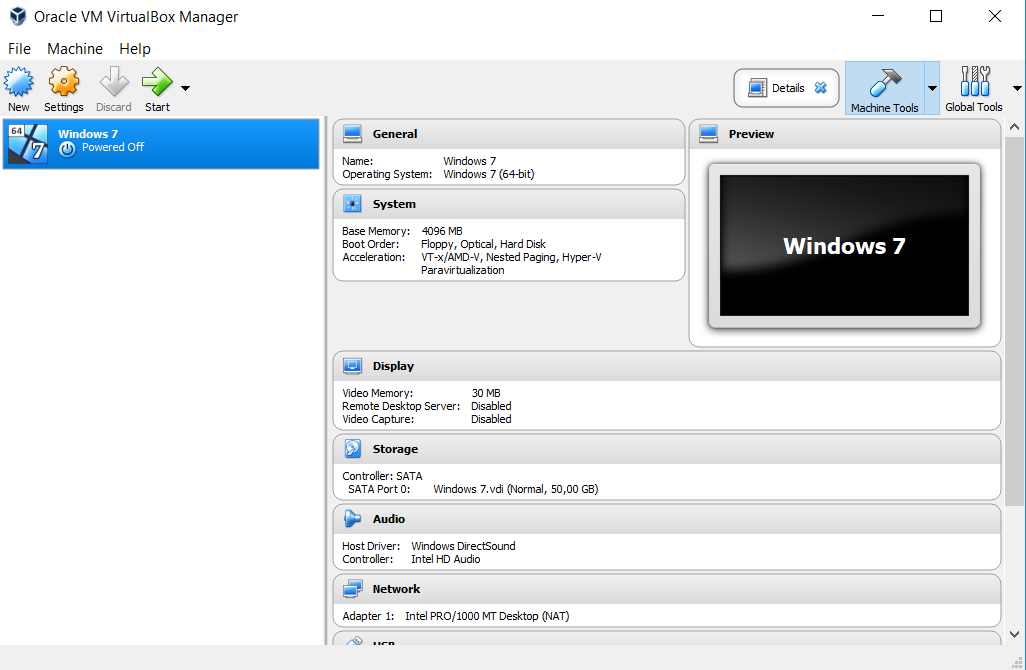
\includegraphics[width=8cm]{chapters/14-vm/img/vbox-main-img.png}
	\caption{Fereastra principală VirtualBox}
	\label{fig:vm-vbox-main}
\end{figure}

Pentru a crea o mașină virtuală nouă mergeți pe meniul Machine -> New. O nouă
fereastră va apărea în care trebuie să introduceți un nume pentru mașina
virtuală precum și tipul sistemului de operare și varianta dorită. În
\labelindexref{Figura}{fig:vm-vbox-create} este exemplificată crearea unei
mașini virtuale ce va rula un sistem de operare Linux, baza pe distribuția
Debian pe 64 de biți.

\begin{figure}[!htbp]
	\centering
	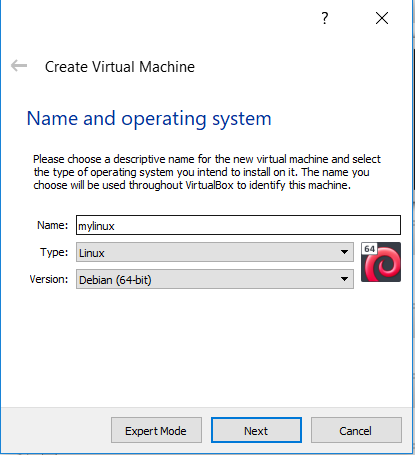
\includegraphics[width=8cm]{chapters/14-vm/img/vbox-create-img.png}
	\caption{Meniul de creare a unei mașini virtuale}
	\label{fig:vm-vbox-create}
\end{figure}

După selectarea sistemului de operare, trebuie să specificați cantitatea de
memorie la care va avea acces mașina virtuală (poate fi modificată și după
creare) precum și dimensiunea discului unde se va instala sistemul de operare.
Există trei tipuri de discuri: VDI (specific VirtualBox), VHDX (specific
Hyper-V), VMDK (specific VMware). Recomandăm folosirea tipului de disc specific
VirtualBOX (VDI) întrucât aceasta va fi aplicația folosită. După selectarea
tipului discului, avem două alte opțiuni:

\begin{itemize}
	\item Fixed size (dimensiune fixă): tot spațiul va fi alocat pe disc de
		la crearea mașinii virtuale. Acest mod oferă performanță mai
		bună, dar spațiul trebuie să fie disponibil de la creare.
	\item Dynamically allocated (alocat dinamic): spațiul va fi alocat pe
		disc pe măsură ce mașina virtuală va scrie date. În acest fel
		putem crea discuri oricât de mari la început, fără să avem
		spațiu disponibil pe discul fizic.
\end{itemize}

În ultimă instanță trebuie să specificați dimensiune pe care o doriți pentru
disc. După și acest ecran, mașina virtuală va fi creată. Înainte de a o porni,
trebuie să mai realizăm setări privind rețeaua. Executați \textit{Right-click}
pe mașina virtuală creată și apăsați pe butonul \textit{Settings}. În ecranul
nou deschis puteți configura fiecare componentă hardware virtualizată (vezi
\labelindexref{Figura}{fig:vm-vbox-settings}.

\begin{figure}[!htbp]
	\centering
	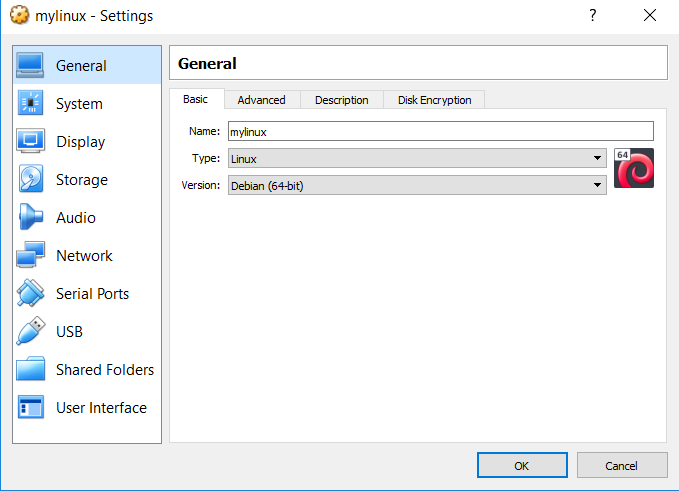
\includegraphics[width=8cm]{chapters/14-vm/img/vbox-settings-img.png}
	\caption{Setările unei mașini virtuale VirtualBox}
	\label{fig:vm-vbox-settings}
\end{figure}

Printre cele mai relevante setări enumerăm:

\begin{itemize}
	\item System - putem configura cantitatea de memoriei, numărul de
		procesoare
	\item Display - cantitatea de memorie utilizată de placa video
	\item Storage - putem vedea ce discuri sunt atașate, ce proprietăți au.
		Tot aici putem adăuga și un disc virtual necesar instalării
		mașinii virtuale. În \labelindexref{Figura}{fig:vm-vbox-iso}
		este reprezentat modul prin care puteți selecta o imagine de tip
		ISO pentru a fi montată ca și un disc virtual în mașina virtuală
		cu scopul de a instala sistemul de operare.
	\item Audio - activare/dezactivare a plăcii audio pentru mașina virtuală
	\item Network - configurarea plăcii/plăcilor de rețea pe care mașina
		virtuală le poate folosi. Implicit doar adaptorul 1
		(\textit{Adapter 1}) este activat și pus în modul NAT (vezi
		\labelindexref{Secțiunea}{sec:vm-ops-config} pentru mai multe
		detalii despre modurile de funcționare). Recomandăm folosirea
		parametrilor impliciți.
	\item USB - configurarea dispozitivelor USB disponibile mașinii
		virtuale. Se poate da acces dispozitivelor USB hardware direct
		mașinii virtuale. Procesul se numește \textit{pass-through}.
\end{itemize}

\begin{figure}[!htbp]
	\centering
	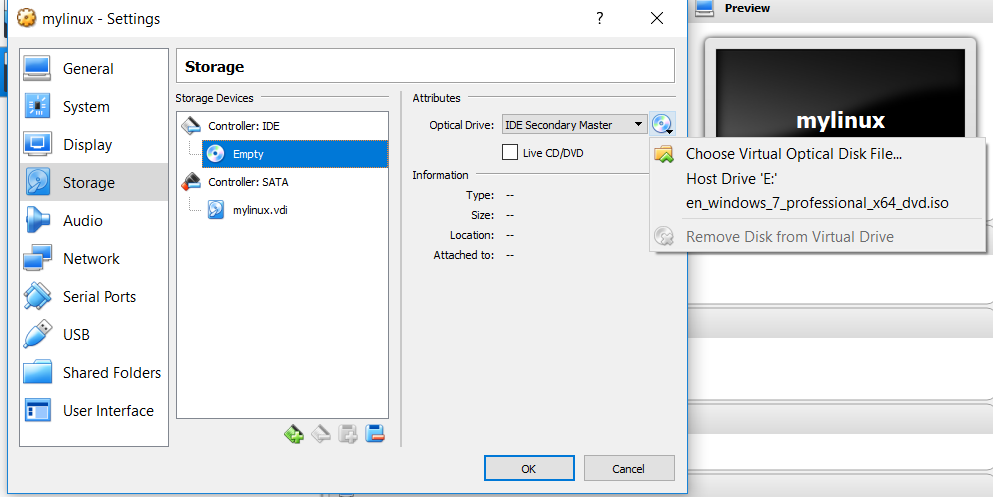
\includegraphics[width=8cm]{chapters/14-vm/img/vbox-iso-img.png}
	\caption{Introducere unei imagini ISO ca disc virtual într-o mașină virtuală}
	\label{fig:vm-vbox-iso}
\end{figure}

După configurarea mașinii virtuale, această poate fi pornită. Selectați mașina
virtuală și apăsați butonul Start din stânga sus. Aceasta va porni și va boota
de pe discul virtual inserat (vezi \labelindexref{Figura}{fig:vm-vbox-iso}). În
\labelindexref{Figura}{fig:vm-vbox-install} este ilustrată pornirea mașinii
virtuale și pornirea sistemului de operare Windows în vedere instalării.

\begin{figure}[!htbp]
	\centering
	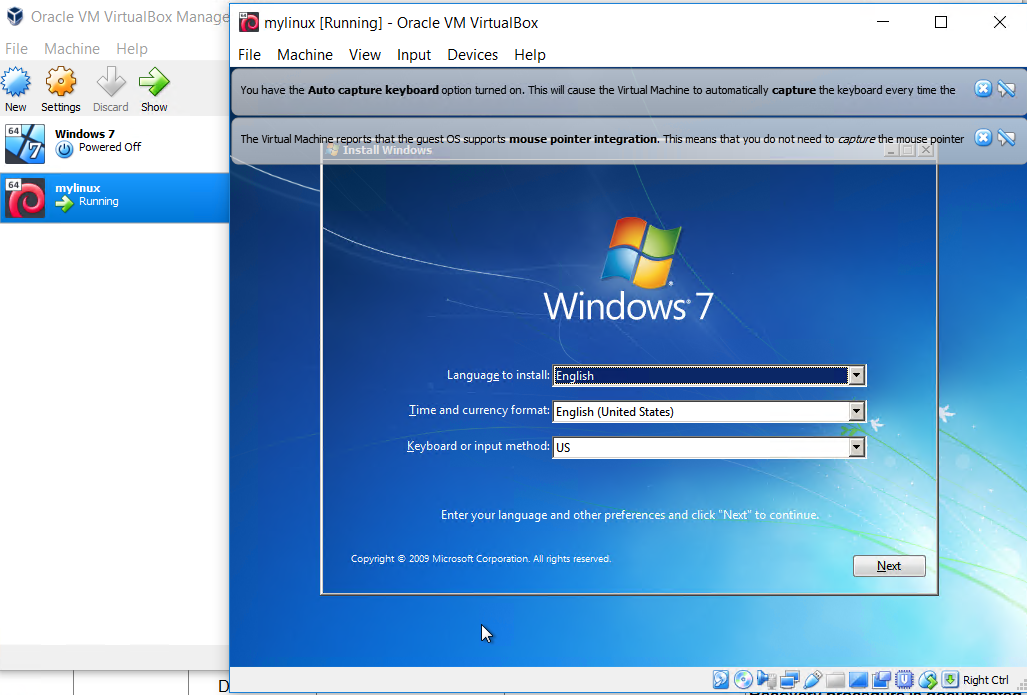
\includegraphics[width=8cm]{chapters/14-vm/img/vbox-install-img.png}
	\caption{Instalarea unui sistem de operare în VirtualBox}
	\label{fig:vm-vbox-install}
\end{figure}

După instalarea sistemului de operare, este important să instalați serviciile de
integrare (vezi \labelindexref{Secțiunea}{sec:vm-ops-services} pentru a întelege
scopul acestora). Pentru a le instala mergeți pe meniul Devices -> Insert Guest
Additions CD Image. Această comandă va monta automat în mașina virtuală un disc
virtual ce conține software-ul de instalat pentru serviciile de integrare. În
\labelindexref{Figura}{fig:vm-vbox-additions} se poate observa noua disc virtual
și conținutul acestuia. De exemplu, după instalarea serviciilor de integrare
veți putea face copy/paste din/în mașina virtuală atât a fișierelor cât și a
textului.

\begin{figure}[!htbp]
	\centering
	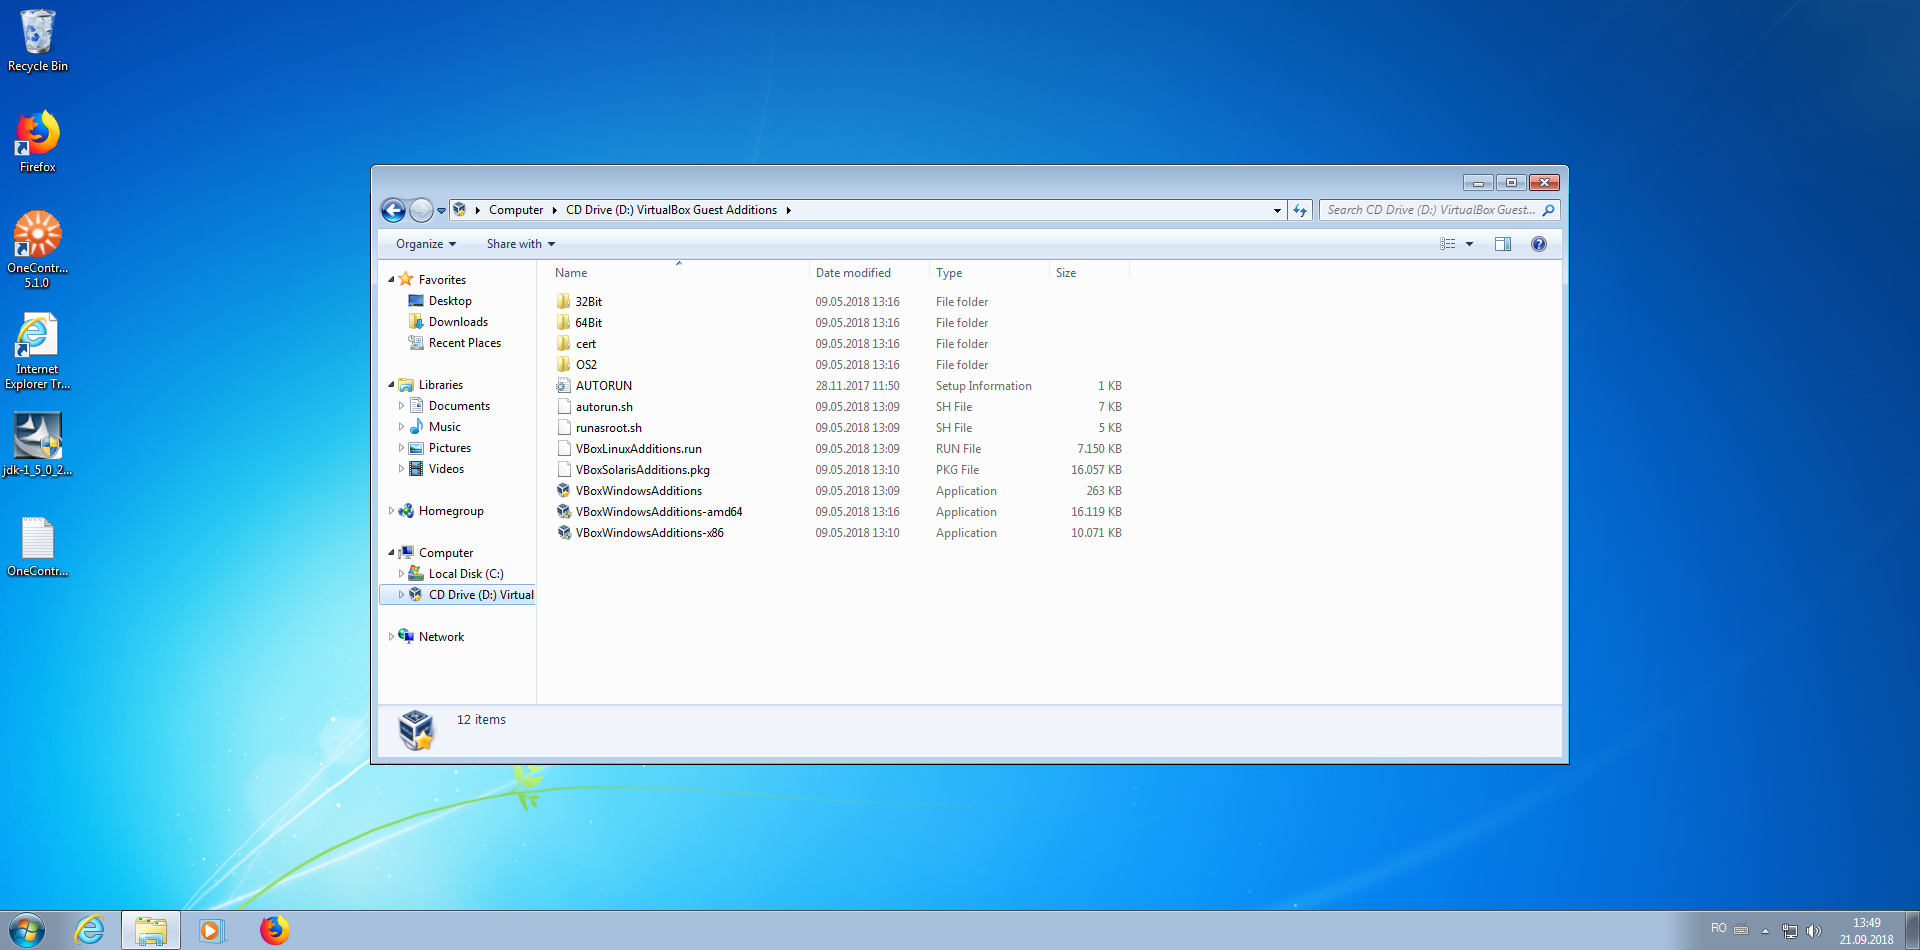
\includegraphics[width=8cm]{chapters/14-vm/img/vbox-additions-img.png}
	\caption{Guest Additions pentru mașini virtuale VirtualBox}
	\label{fig:vm-vbox-additions}
\end{figure}

O operație foarte utilă cu o mașină virtuală este cea de snapshot prezentată și
în \labelindexref{Secțiunea}{sec:vm-ops}. Pentru a realiza acest lucru în
VirtualBox, mergeți pe meniul \textit{Machine tools} din dreapta sus și
selectați butonul \textit{Snapshot}, exact ca în
\labelindexref{Figura}{fig:vm-vbox-snapshot}. Pentru a realiza un snapshot
apăsați butonul \textit{Take}.

\begin{figure}[!htbp]
	\centering
	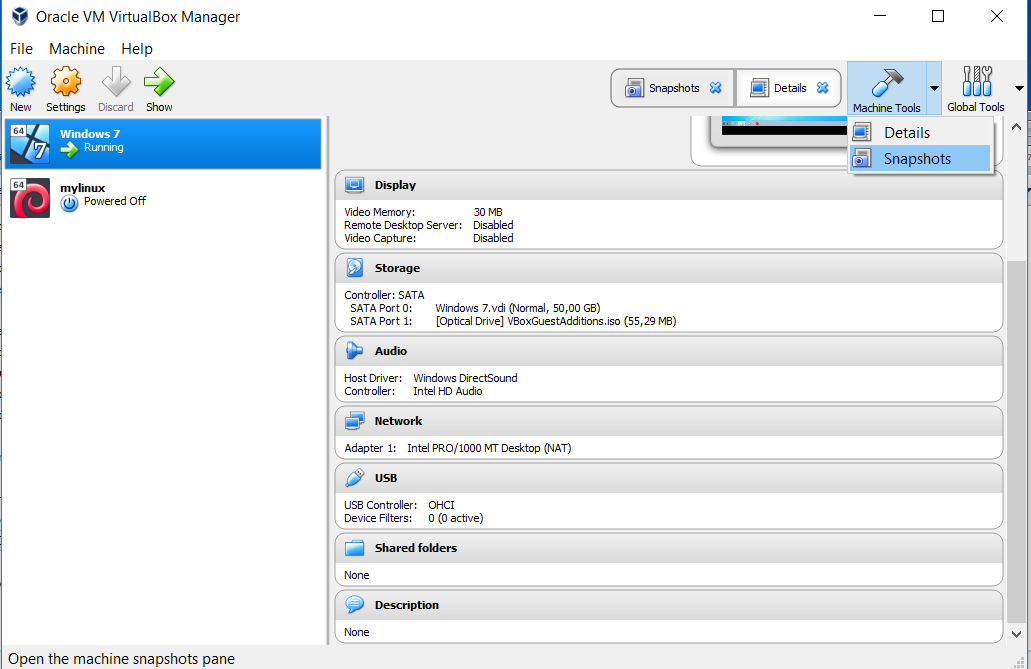
\includegraphics[width=8cm]{chapters/14-vm/img/vbox-snapshot-img.png}
	\caption{Snapshot-ul unei mașini virtuale în VirtualBox}
	\label{fig:vm-vbox-snapshot}
\end{figure}

Va apărea un meniu în care trebuie să introduceți numele snapshotului și o
descriere relevantă. În \labelindexref{Figura}{fig:vm-vbox-view-snapshot} se
poate observa snapshot-ul creat. Pentru a ne întoarce la snapshot-ul dorit,
apăsăm click-dreapta pe mouse pe acesta și selectăm opțiunea \textit{Restore}.
Se poate observa după aceea că mașina a revenit la starea anterioară

\begin{figure}[!htbp]
	\centering
	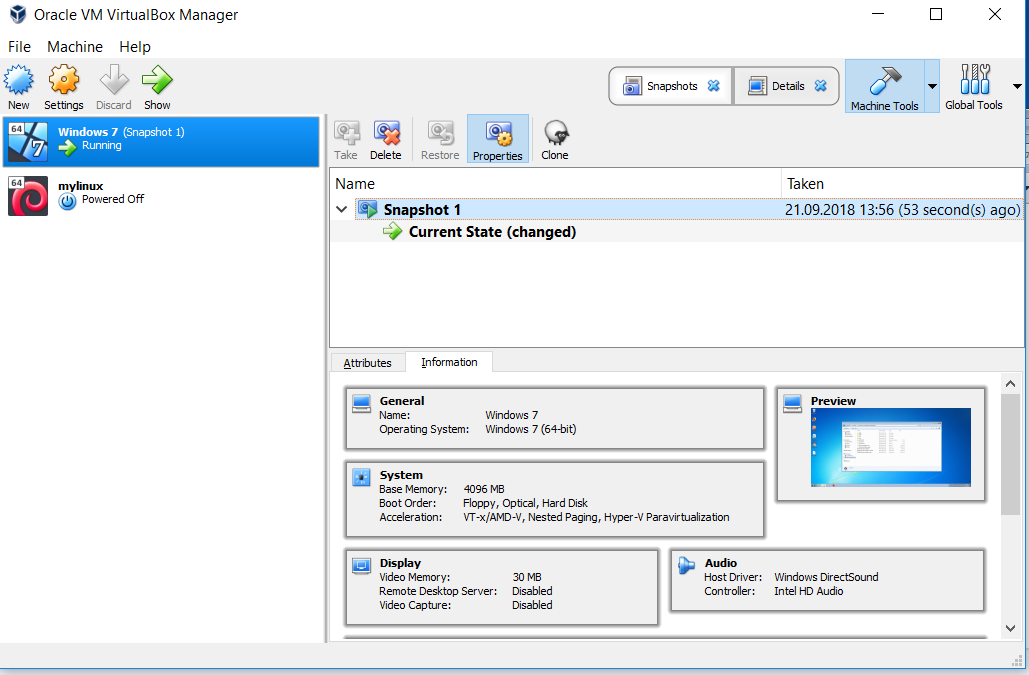
\includegraphics[width=8cm]{chapters/14-vm/img/vbox-view-snapshot-img.png}
	\caption{Snaptshot creat în cadrul VirtualBox}
	\label{fig:vm-vbox-view-snapshot}
\end{figure}

\section{Anexă: Openstack în UPB}
\label{sec:vm-openstack}

Din perspectiva Openstack, un student face parte dintr-un tenant (vezi
Multitenancy). În acest context, noțiunea de tenant poate fi asociata cu un
proiect. Crearea proiectului se face prin apăsarea butonului Create user, buton
aflat în blocul Openstack de pe platforma Moodle a Facultății de Automatică și
Caculatoare (acs.curs.pub.ro - acest lucru este specific doar pentru studenții
facultății, vezi \labelindexref{Figura}{fig:vm-openstack-project}). Odată
tenant-ul creat, putem accesa Dashboard pentru crearea mașinilor virtuale.

\begin{figure}[!htbp]
	\centering
	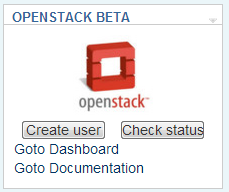
\includegraphics[width=8cm]{chapters/14-vm/img/openstack-project-img.png}
	\caption{Crearea proiect Openstack}
	\label{fig:vm-openstack-project}
\end{figure}

\subsection{Accesarea Openstack Dashboard}
\label{sec:vm-openstack-dashboard}

Interfața de administrare a Openstack (Openstack Dashboard) se poate accesa
folosind link-ul https://cloud-controller.grid.pub.ro/. Autentificarea se face
folosind utilizatorul și parola furnizate de către facultate.

\begin{figure}[!htbp]
	\centering
	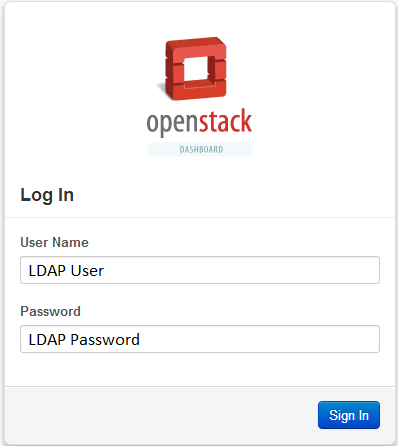
\includegraphics[width=8cm]{chapters/14-vm/img/openstack-dashboard-img.png}
	\caption{Dashboard-ul Openstack}
	\label{fig:vm-openstack-dashboard}
\end{figure}

\subsection{Crearea unei perechi de chei ssh publica-privata}
\label{sec:vm-openstack-keys}

Autentificarea în cadrul unei mașini virtuale se face folosind ssh cu chei
publice-private. Acest mod de autentificare asigură cel mai înalt grad de
securitate fiind folosit și de Amazon EC2 în mod implicit. Generarea de chei se
va face pe fep.grid.pub.ro astfel

\begin{screen}
ssh ldap_user@fep.grid.pub.ro
mkdir .ssh
cd .ssh
ssh-keygen -t rsa -b 2048 -f openstack.key -C "openstack-ssh-key"
\end{screen}

În acest moment în directorul ~/.ssh ar trebui sa existe 2 fișiere:

\begin{itemize}
	\item openstack.key -- cheia privata
	\item openstack.key.pub -- cheia publica
\end{itemize}

\subsection{Crearea unui keypair}
\label{sec:vm-openstack-keypares}

Un keypair reprezinta o asociere între un nume și o cheie publică. În Openstack,
cheia publică se va identifica printr-un nume, specificat la creare. Cheia
publică creată la pasul anterior trebuie încărcată în Openstack. Acest lucru se
face din Openstack Dashboard -> Project -> Compute -> Access \& Security -> Key
Pairs -> Import Key Pair (vezi \labelindexref{Figura}{fig:vm-openstack-keypair}).

\begin{figure}[!htbp]
	\centering
	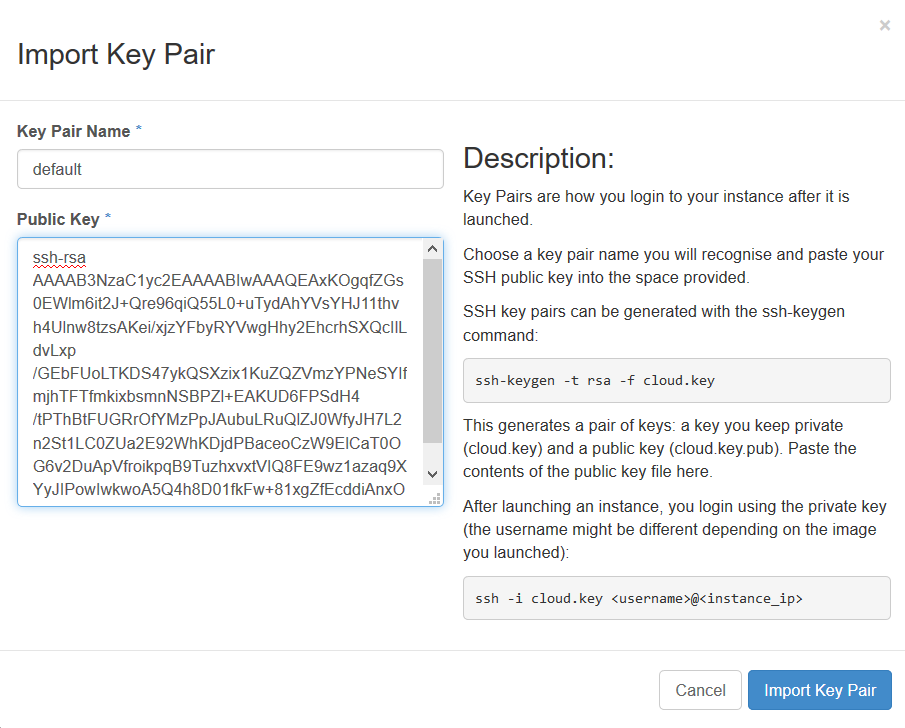
\includegraphics[width=8cm]{chapters/14-vm/img/openstack-keypair-img.png}
	\caption{Alegerea unui keypair la crearea unei instanțe}
	\label{fig:vm-openstack-keypair}
\end{figure}

\subsection{Crearea unei mașini virtuale}
\label{sec:vm-openstack-createvm}

Crearea unei masini virtuale se poate face atât din Openstack Dashboard cât și
din linia de comandă. În acest tutorial va fi prezentată varianta folosind
Openstack Dashboard. Pentru a lansa o instanță, accesați Openstack Dashboard ->
Project -> Compute -> Instances -> Launch Instance (vezi
\labelindexref{Figura}{fig:vm-openstack-info-img})

\begin{figure}[!htbp]
	\centering
	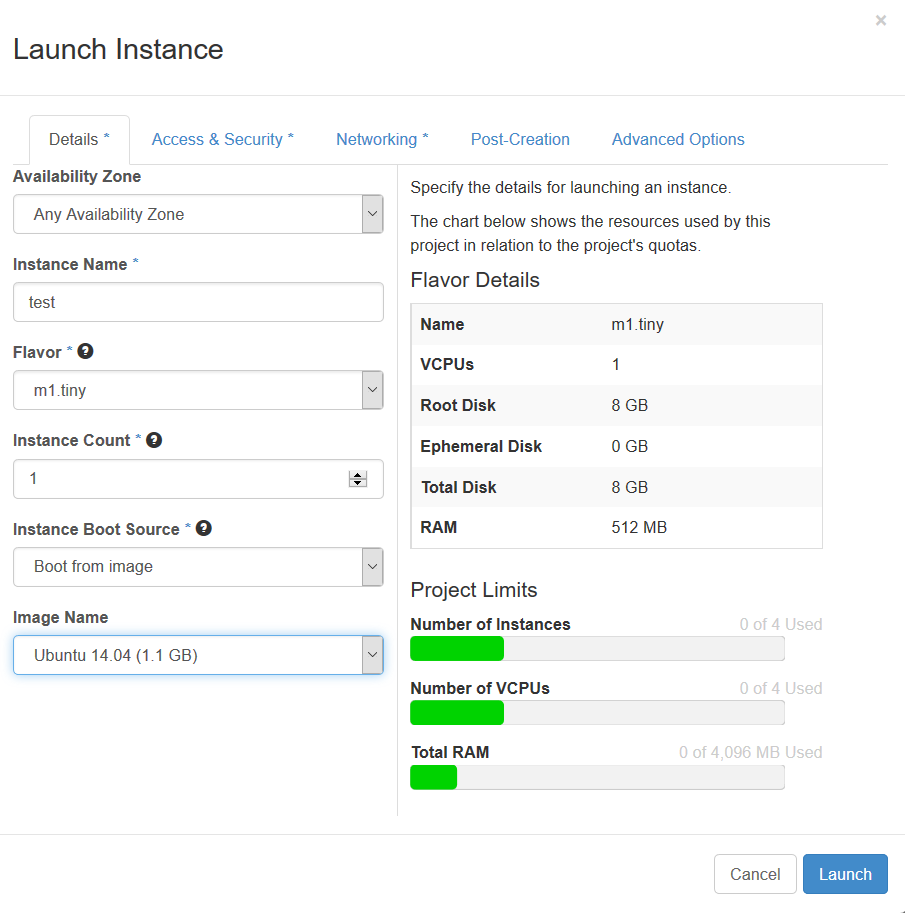
\includegraphics[width=8cm]{chapters/14-vm/img/openstack-info-img.png}
	\caption{Crearea unei instanțe Openstack}
	\label{fig:vm-openstack-info-img}
\end{figure}

În exemplul de față, am folosit template-ul “Ubuntu 14.04”. Un flavor reprezinta
mărimea unei instanțe virtuale din punct de vedere al resurselor: număr de
procesoare, memorie și spatiu pe disk. Din tabul Access \& Security, alegeți
Keypair-ul creat anterior (vezi
\labelindexref{Figura}{fig:vm-openstack-keychoice}). În final, apăsați pe Launch
pentru a crea mașina virtuală.

\begin{figure}[!htbp]
	\centering
	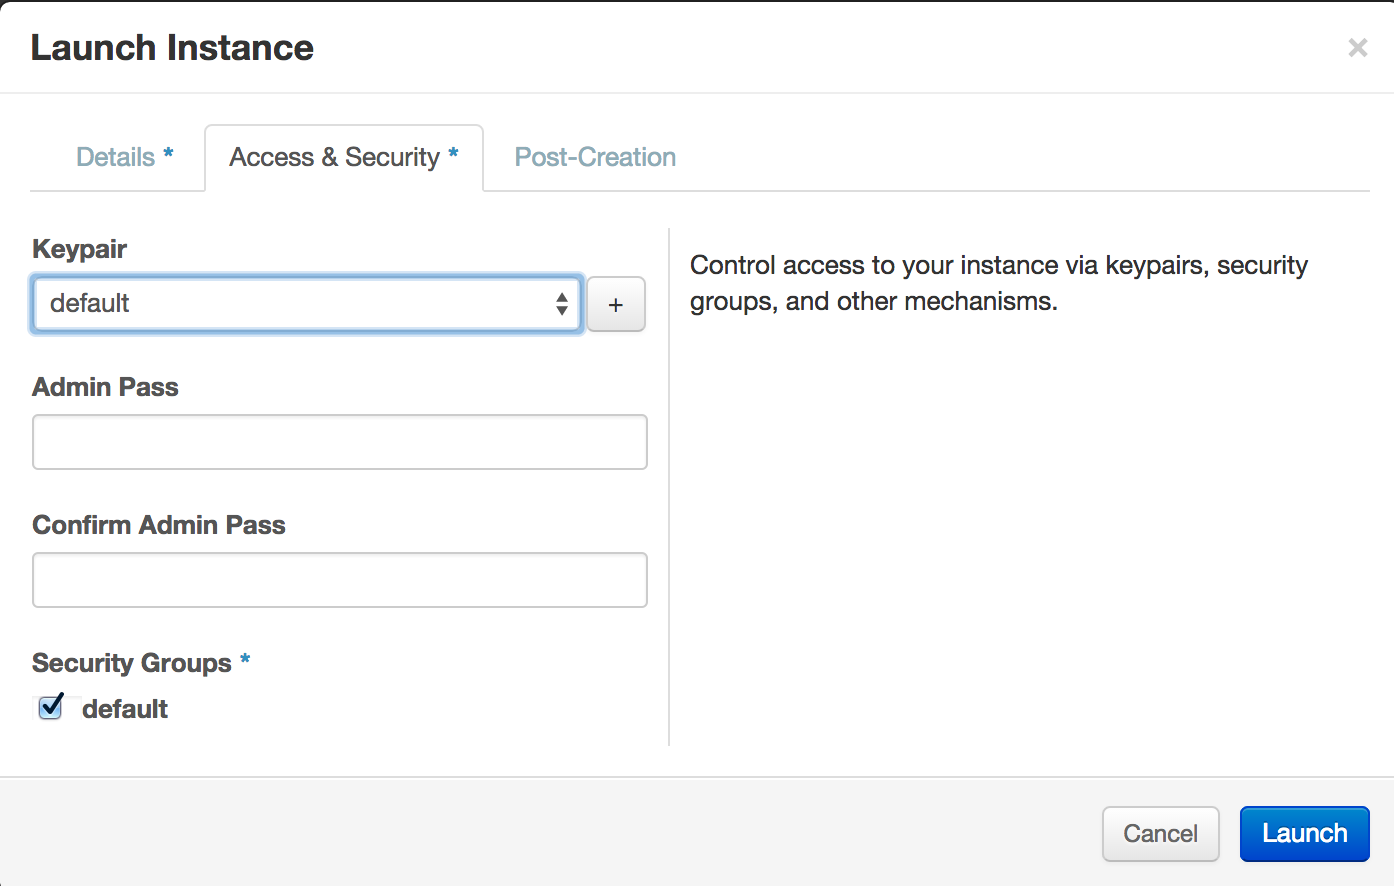
\includegraphics[width=8cm]{chapters/14-vm/img/openstack-keychoice-img.png}
	\caption{Importarea unei perechi de chei în Openstack}
	\label{fig:vm-openstack-keychoice}
\end{figure}

\subsection{Accesarea masinii virtuale}
\label{sec:vm-openstack-accessvm}

Accesarea mașinii virtuale se va face prin ssh de pe fep.grid.pub.ro astfel:

\begin{screen}
ssh ldap_user@fep.grid.pub.ro
ssh -i ~/.ssh/openstack.key student@10.9.0.138 #(in cazul de fata)
\end{screen}

\begin{figure}[!htbp]
	\centering
	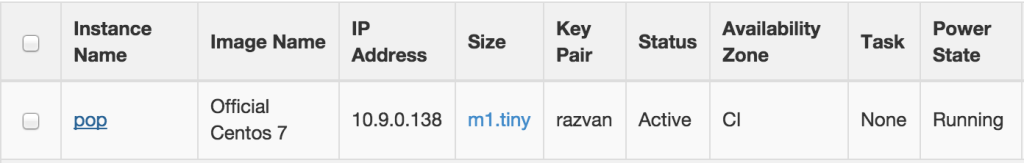
\includegraphics[width=8cm]{chapters/14-vm/img/openstack-short-info-img.png}
	\caption{Informații despre mașina virtuală}
	\label{fig:vm-openstack-info}
\end{figure}

Adresa IP 10.9.0.138 reprezintă adresa publică a mașinii virtuale (vezi
\labelindexref{Figura}{fig:vm-openstack-info}). O mașină virtuală se va accesa
întotdeauna folosind adresa publică. Aceasta va fi din clasa 10.9.0.0/16 în
cazul instalării Openstack din facultate. Utilizatorul folosit la autentificare
este student. Pentru alte template-uri gasiti aici lista cu username-urile
pentru fiecare template:
https://cloud.curs.pub.ro/2014/12/17/username-uri-implicite/.

\subsection{Ștergerea masinii virtuale}
\label{sec:vm-openstack-deletevm}

Odata ce ați finalizat procesul de folosire a mașinii virtuale trebuie să o
ștergeți pe aceasta. Acest lucru se face folosind butonul Terminate Instance,
după ce ați selectat instanța pe care doriți să o ștergeți. În urma apăsării
butonului Terminate Instance toate datele stocate în acea instanță se vor
pierde.

\section{Anexă: Rularea unui sistem de operare compilat pentru ARM pe x86}
\label{sec:vm-arm}

Pentru rularea unui sisteme de operare compilat pentru arhitectura ARM pe un
sistem de operare ce rulează pe o arhitectură x86, avem nevoie de un emulator.
Vom folosi emulatorul qemu ce are suportul de emulare pentru arhitectura ARM.
Vom instala aplicația (comanda este validă pe un sistem Debian-based):

\begin{screen}
student@uso~:$ sudo apt-get install qemu qemu-kvm qemu-system-arm
\end{screen}

Pentru a rula un sistem de operare, avem nevoie de un nucleu (kernel) precum și
de un binarele aferente (sistemul de fișiere). O imagine de kernel Linux pentru
arhitectura ARM se poate descărca de la adresa
http://uso.cs.pub.ro/virtualizare/kernel-qemu. Pentru sistemul de fișiere vom
folosi o imagine de numită Raspbian (mașină virtuală de Debian care merge pe un
sistem de fișiere tip Raspberry Pi), descărcabilă de la adresa
http://uso.cs.pub.ro/virtualizare/2012-10-28-wheezy-raspbian.zip. După ce
descăcați fișierul, îl dezarhivați pentru a obține sistemul de fișiere. Vom
porni sistemul de operare folosind următoarea comandă:

\begin{screen}
student@uso~:$ qemu-system-arm -kernel kernel-qemu -cpu arm1176 -m 256 -M versatilepb -no-reboot -serial stdio -append "root=/dev/sda2 panic=1 rootfstype=ext4 rw" -hda 2012-10-28-wheezy-raspbian.img
\end{screen}

Printre parametrii relevanți folosiți în comandă, putem enumera:

\begin{itemize}
	\item -kernel - specifică imaginea de kernel de va rula
	\item -cpu - specifică modelul procesorului pe care îl va emula
	\item -m - definește cantitatea de memorie ce va fi alocată
	\item -hda - specifică imaginea sistemului de fișiere ce va fi utilizată
\end{itemize}


În \labelindexref{Figura}{fig:vm-qemu-bootup} se observă cum booteză sistemul de
operare emulat. Pornirea acestuia durează în jur de 60 de secunde, mai lent
decât pornirea unei mașini virtuale (30 secunde).

\begin{figure}[!htbp]
	\centering
	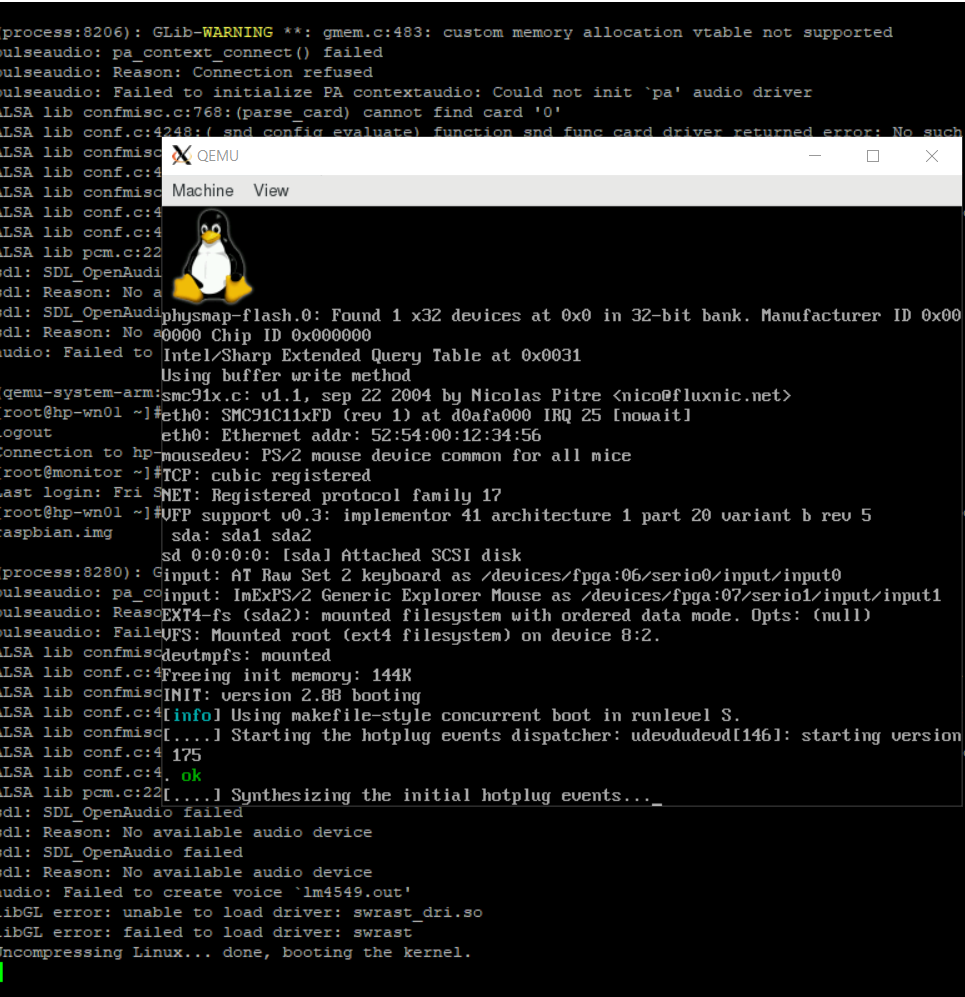
\includegraphics[width=8cm]{chapters/14-vm/img/qemu-bootup-img.png}
	\caption{Pornirea unui sistem de operare emulate}
	\label{fig:vm-qemu-bootup}
\end{figure}

Pentru a vă autentifica în consola sistemului de operare emulat, folosiți
utilizatorul \textit{pi} și parola \textit{raspberry}:

\begin{screen}
raspberry pi login: pi
Password:
...
pi@raspberrypi:~$
\end{screen}


Dorim să comparăm performanța unui sistem virtualizat cu ce a unuia emulat. Vom
considera următorul fișer sursă:

\begin{screen}
int main()
{
    int i;


    for (i=0; i<1000000; i++)
        i++;
}
\end{screen}

Vom măsura durata timpului de compilare pe un sistem emulat:

\begin{screen}
pi@raspberrypi:~$ time gcc test.c


real    0m1.103s
user    0m0.800s
sys     0m0.280s
\end{screen}

Pentru un sistem virtualizat durata compilării este:

\begin{screen}
[root@monitor ~]# time gcc test.c


real    0m0.077s
user    0m0.036s
sys     0m0.028s
\end{screen}

Se observă că pe un sistem de operare virtualizat, operația de compilare s-a
executat mult mai rapid (a durat 77ms), iar pe un sistem emulat a durat
compilarea aceluiași fișier mai mult de o secundă. Acest lucru se întâmplă din
cauza faptului că fiecare instrucțiuni trebuie interpretată de către emulator.
